\chapter{Descripci\'{o}n general de la investigaci\'{o}n}
\label{chap:descripcion}
\epigraph{Simplicity is prerequisite for reliability.}{Edsger W. Dijkstra}

En este cap\'{i}tulo se describe la investigaci\'{o}n realizada. Primero se brinda la hip\'{o}tesis, la cual propone que es posible reconstruir r\'{a}pidamente un objeto tridimensional del mundo real a partir de informaci\'{o}n contenida en im\'{a}genes capturadas con equipo barato, como es el caso de c\'{a}maras \textit{webcam}. Seguidamente, se detalla el experimento realizado para comprobar dicha hip\'{o}tesis. El experimento consta de una c\'{a}mara barata, una base giratoria de madera y la t\'{e}cnica de reconstrucci\'{o}n r\'{a}pida propuesta en esta tesis. Finalmente, se brinda una secci\'{o}n de aportes, alcances y limitaciones de dicha t\'{e}cnica.


\section{Hip\'{o}tesis}
La hip\'{o}tesis que defiende esta tesis dice que \textbf{es posible reconstruir r\'{a}pidamente un objeto tridimensional a partir de, \'{u}nicamente, la informaci\'{o}n contenida en una secuencia de im\'{a}genes que provienen de una c\'{a}mara convencional de bajo costo y utilizando una serie de t\'{e}cnicas del campo de la visi\'{o}n artificial.}


\section{Descripci\'{o}n general de la t\'{e}cnica}
La t\'{e}cnica presentada en esta tesis se basa en el mecanismo de estructura a partir del movimiento (del ingl\'{e}s \textit{structure from motion}), proceso que involucra estimar simult\'{a}neamente la geometr\'{i}a 3D (estructura) y la posici\'{o}n de la c\'{a}mara (movimiento) \cite{Ullman_1979,Szeliski_2010,Hartley_Zisserman_2003}. La t\'{e}cnica permite convertir r\'{a}pidamente pares de im\'{a}genes estereosc\'{o}picas bidimensionales de un objeto del mundo real en una representaci\'{o}n tridimensional de \'{e}ste, conocida como nube densa de puntos 3D.

La conversi\'{o}n de im\'{a}genes bidimensionales en una representaci\'{o}n tridimensional se inicia con una fase de calibraci\'{o}n de la c\'{a}mara, para determinar sus par\'{a}metros intr\'{i}nsecos y extr\'{i}nsecos. Posteriormente, se procede a aplicar una t\'{e}cnica pir\'{a}mide a las im\'{a}genes para reducir su procesamiento. Seguidamente, se realiza un rastreo denso y un pareo de pixeles entre cada par de im\'{a}genes estereosc\'{o}picas con tal de determinar su desplazamiento. Para lograr esto, se cre\'{o} un algoritmo de pareo denso basado en la detecci\'{o}n del flujo \'{o}ptico en lugar del tradicional pareo de caracter\'{i}sticas sobresalientes. Finalmente, se procede a determinar la profundidad calculando el movimiento entre c\'{a}maras (vistas) y luego triangulando los puntos del objeto utilizando el algoritmo iterativo de m\'{i}nimos cuadrados presentado en \cite{hartley1997triangulation}. En la figura ~\ref{fig:SystemOverview} se muestra el esquema general de la t\'{e}cnica r\'{a}pida de reconstrucci\'{o}n tridimensional.


\begin{figure}[H]
\centering
\includegraphics[width=1.0\textwidth]{images/systemoverview.png}
\caption[Esquema general de la t\'{e}cnica r\'{a}pida de reconstrucci\'{o}n tridimensional]%
{Esquema general de la t\'{e}cnica r\'{a}pida de reconstrucci\'{o}n tridimensional. Imagen creada por el autor de este documento.}
\label{fig:SystemOverview}
\end{figure}


Las fases de refinamiento, registro, \textit{meshing} y reconstrucci\'{o}n de la superficie no se contemplan en esta tesis pero pueden ser explorados en trabajo futuro.

\section{Descripci\'{o}n general del experimento}
Para el experimento se utilizaron dos c\'{a}maras tipo \textit{webcam} de bajo costo. La primera es una c\'{a}mara estereosc\'{o}pica con un sensor de baja definici\'{o}n conocida como \textit{Minoru 3D Webcam}. Creada en el 2009 por la compa\~n\'{i}a \textit{Promotion and Display Technology of Salford, Greater Manchester}, esta c\'{a}mara posee 2 sensores VGA de 640x480 y es capaz de capturar im\'{a}genes con resoluciones que van desde 320x240 hasta un m\'{a}ximo de 800x600. El monto invertido en la compra de la c\'{a}mara fue de \$21.42 en el a\~no 2011. En la figura ~\ref{fig:Camera1} se muestra esta c\'{a}mara.


\begin{figure}[H]
\centering
\includegraphics[width=0.7\textwidth]{images/camara1.jpg}
\caption[Minoru 3D Webcam]%
{La \textit{Minoru 3D Webcam} es una c\'{a}mara estereosc\'{o}pica de muy bajo costo que permite capturar im\'{a}genes 2D y 3D. M\'{a}s informaci\'{o}n en \url{http://www.minoru3d.com}.}
\label{fig:Camera1}
\end{figure}


La segunda es una c\'{a}mara con un lente de alta definici\'{o}n conocida como \textit{Logitech Webcam Pro C910}. Creada en el 2012 por la compa\~n\'{i}a \textit{Logitech}, esta c\'{a}mara posee un sensor de alta definici\'{o}n y un lente tipo \textit{Carl Zeiss\footnote{Carl Zeiss fue un alem\'{a}n que vivi\'{o} del a\~no 1816 al 1888, el cual fund\'{o} la compa\~n\'{i}a \textit{Carl Zeiss Jena} (ahora \textit{Carl Zeiss AG}). Para m\'{a}s informaci\'{o}n visitar \url{http://www.zeiss.com}} Tessar}\copyright el cual est\'{a} considerado como uno de los lentes de mayor calidad que existe en el mercado. Es capaz de capturar im\'{a}genes con resoluciones que van desde 160x120 hasta un m\'{a}ximo de 2592x1944. El monto invertido en la compra de la c\'{a}mara fue de \$70.62 en el a\~no 2011. En la figura ~\ref{fig:Camera2} se muestra esta c\'{a}mara.


\begin{figure}[H]
\centering
\includegraphics[width=1.0\textwidth]{images/camara2.jpg}
\caption[Logitech Webcam Pro C910]%
{La \textit{Logitech Webcam Pro C910} tiene un lente \textit{Carl Zeiss Tessar}\copyright y un sensor de alta definici\'{o}n. Más información en \url{http://www.logitech.com}.}
\label{fig:Camera2}
\end{figure}


Para realizar la reconstrucci\'{o}n, se posiciona una de las c\'{a}maras de forma fija a una distancia que permita observar gran parte o la totalidad del objeto a reconstruir. El objeto se posiciona sobre una base giratoria similar a la que se muestra en la figura ~\ref{fig:Base} y finalmente, se ejecuta el experimento utilizando una computadora personal. La luz afecta considerablemente la calidad de la reconstrucci\'{o}n, por lo que se recomienda que la base giratoria y el objeto se posicionen en un lugar con suficiente iluminaci\'{o}n.


\begin{figure}[H]
\centering
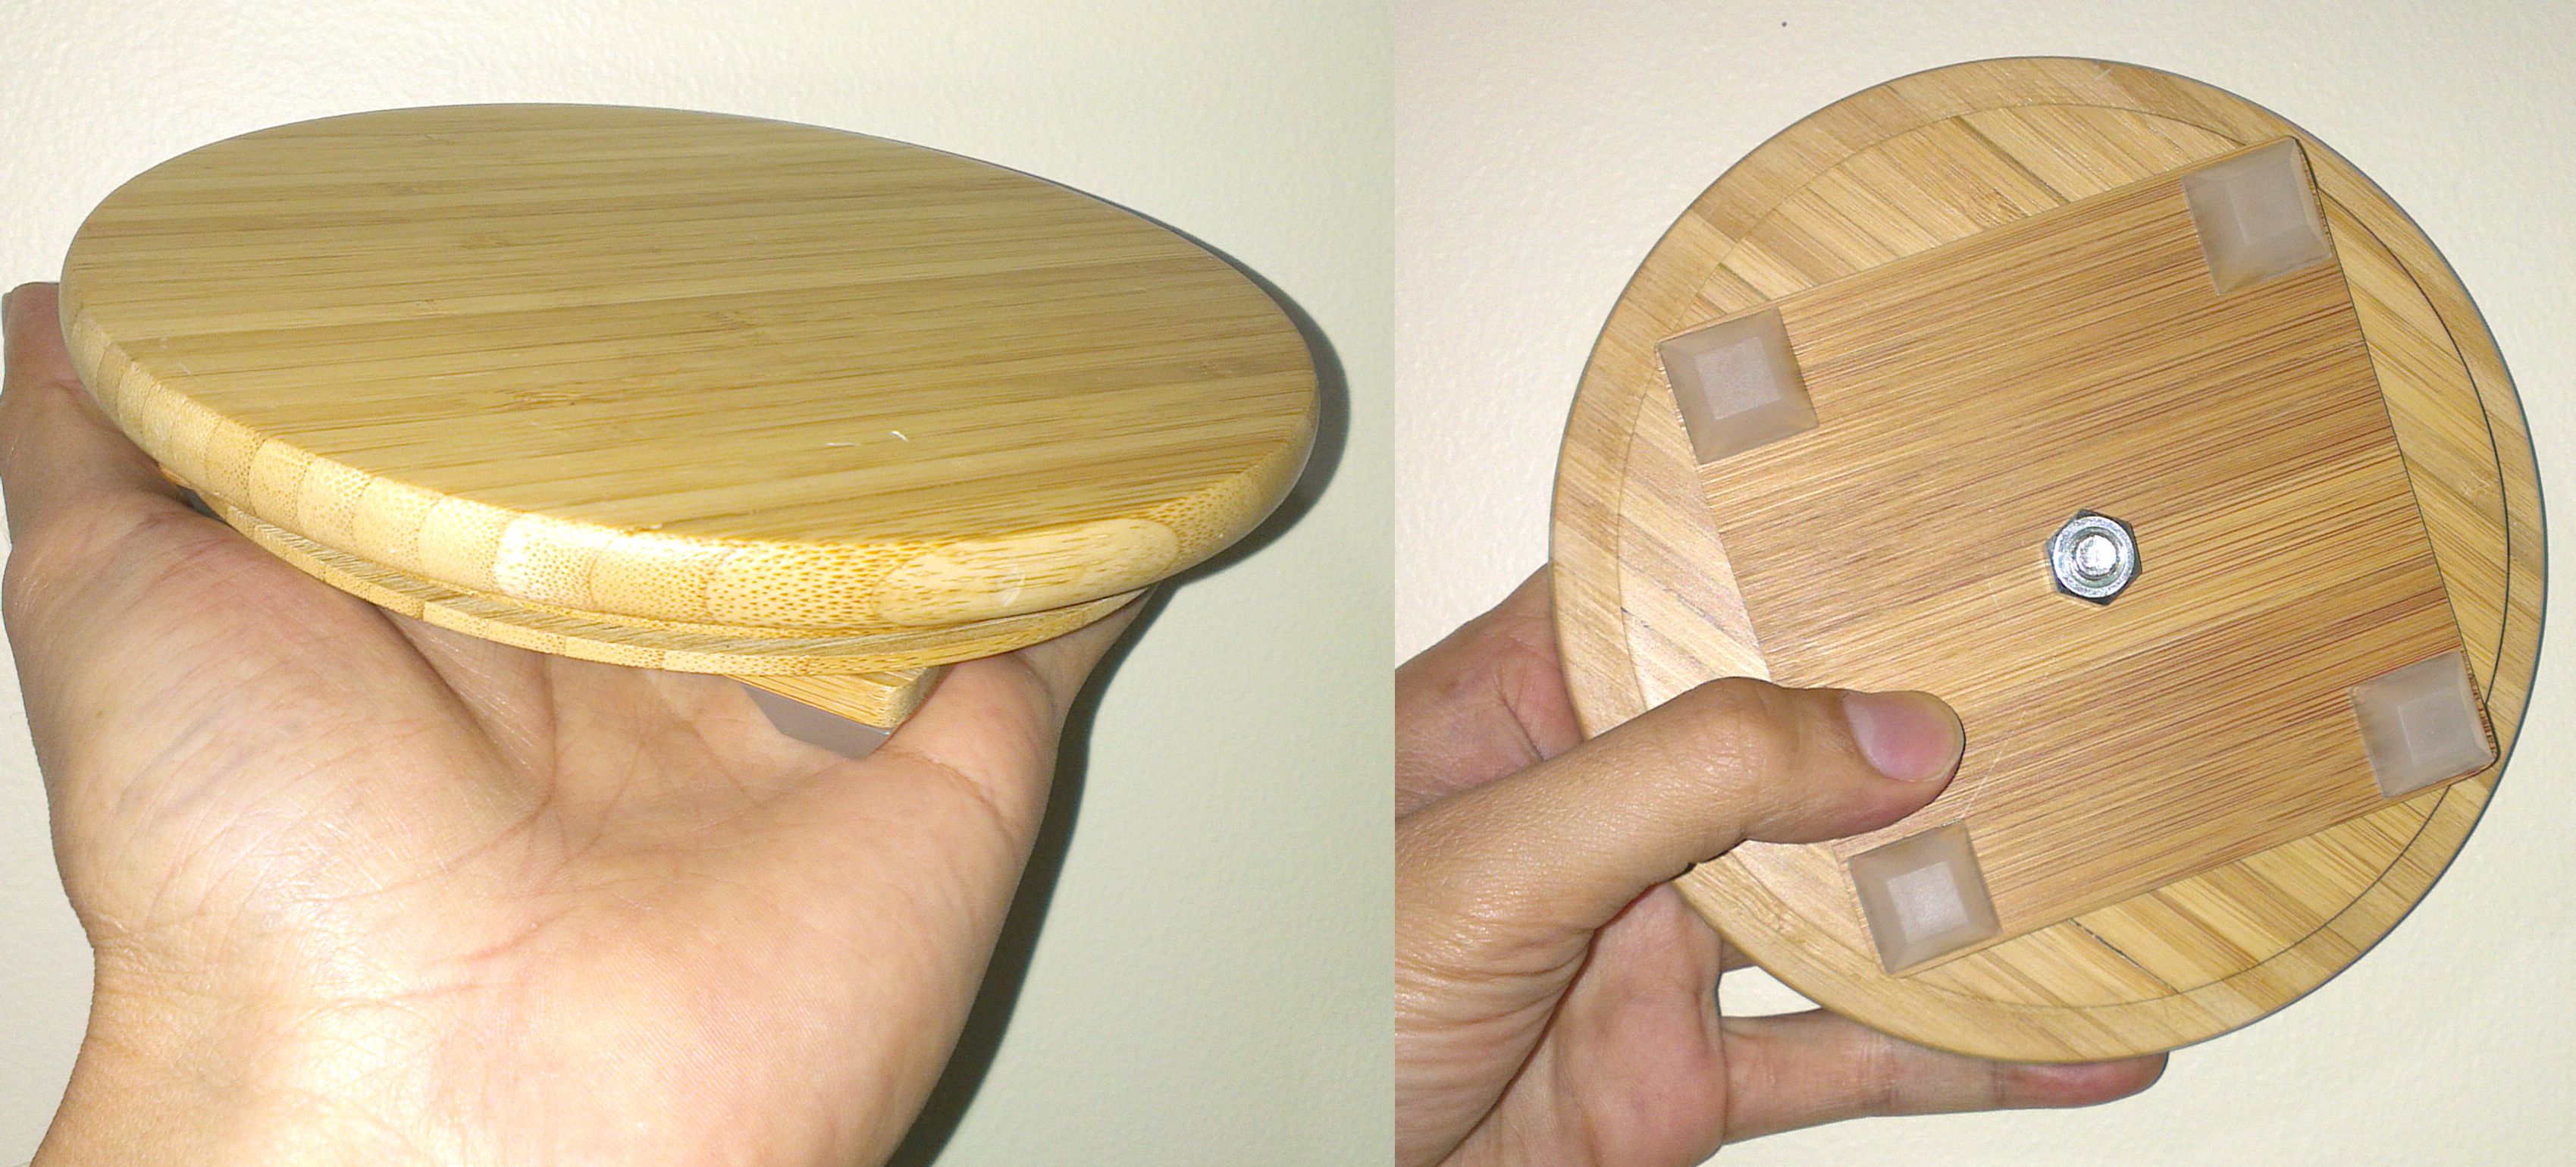
\includegraphics[width=1.0\textwidth]{images/base1.png}
\caption[Base giratoria]%
{Base giratoria hecha de una tapa de un envase de cocina, un rol de patineta, un portavasos de madera y un tornillo con tuerca. Monto total invertido en la construcci\'{o}n de la base: \$6.}
\label{fig:Base}
\end{figure}


No se hace ning\'{u}n tipo de suposici\'{o}n acerca de la geometr\'{i}a del objeto y no se conoce ning\'{u}n tipo de informaci\'{o}n del objeto \textit{a priori}. El \'{u}nico requerimiento particular de la t\'{e}cnica es la necesidad de que el objeto sea r\'{i}gido\footnote{Enti\'{e}ndase r\'{i}gido como un objeto cuya estructura geom\'{e}trica no var\'{i}a de una imagen a otra.} y que su textura no sea muy uniforme.


\begin{figure}[H]
\centering
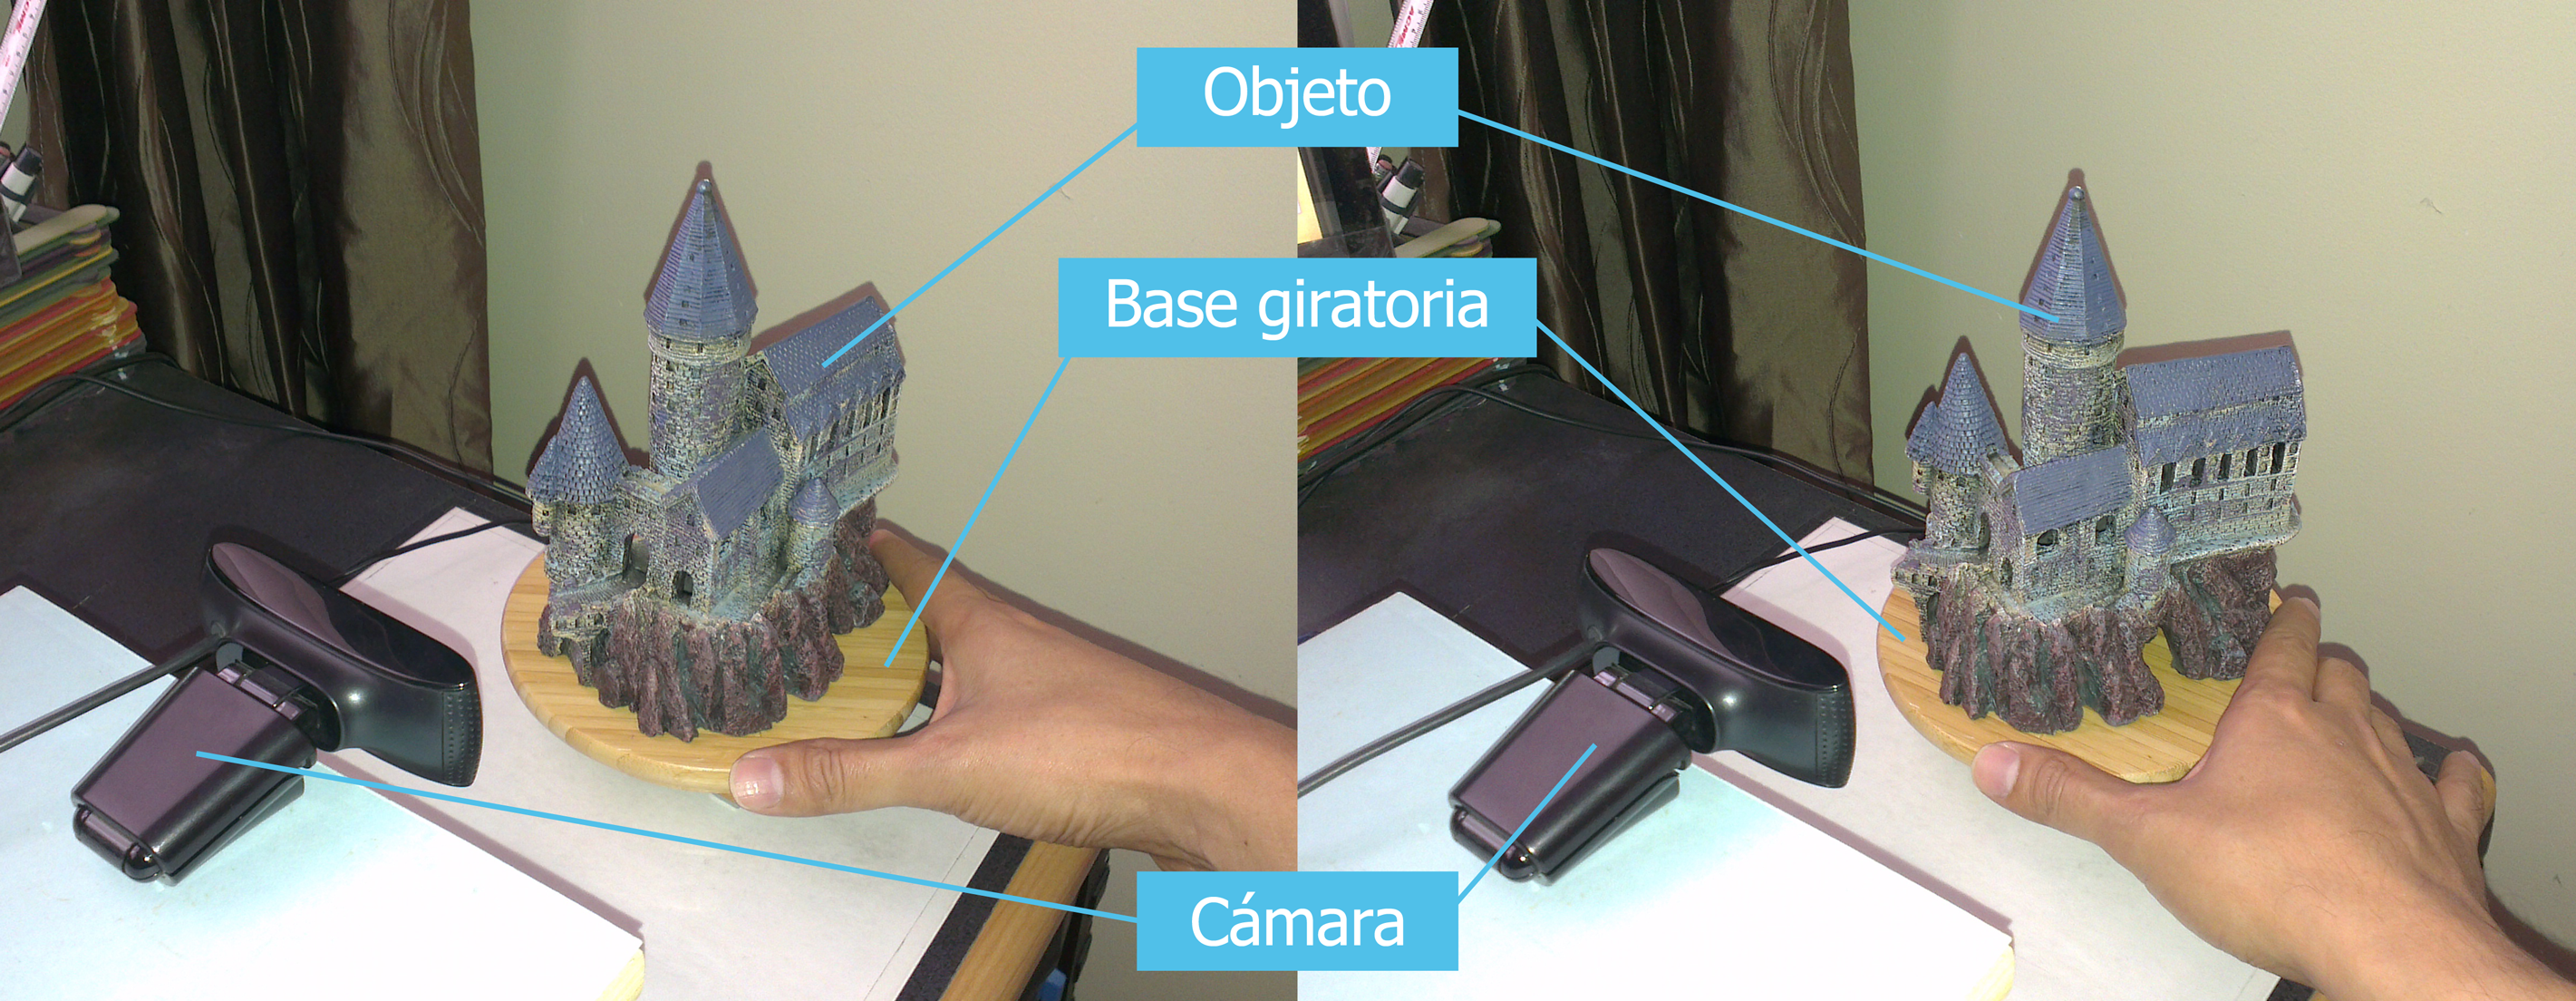
\includegraphics[width=1.0\textwidth]{images/so.png}
\caption[Sistema completo utilizado para el experimento de la t\'{e}cnica r\'{a}pida de reconstrucci\'{o}n tridimensional]%
{Sistema completo utilizado para el experimento de la t\'{e}cnica r\'{a}pida de reconstrucci\'{o}n tridimensional. El sistema est\'{a} compuesto por una c\'{a}mara tipo \textit{webcam}, una base giratoria, el objeto a reconstruir y una computadora personal donde ejecutar los algoritmos.}
\label{fig:SO}
\end{figure}


Como se muestra en la figura ~\ref{fig:SO}, conforme el objeto va rotando frente a la c\'{a}mara, se toma una serie de vistas clave (del ingl\'{e}s \textit{keyframes}) para realizar la auto calibraci\'{o}n del sistema. Posteriormente, se procede con la fase r\'{a}pida de estimaci\'{o}n del movimiento en la cual se determinan los valores necesarios para reconstruir la posici\'{o}n y orientaci\'{o}n de la c\'{a}mara. Finalmente, se procede con la fase de recuperaci\'{o}n de la profundidad v\'{i}a el algoritmo iterativo de triangulaci\'{o}n. El resultado final es la representaci\'{o}n tridimensional del objeto en forma de una nube coloreada de puntos 3D. Todo el proceso toma unos cuantos segundos.




\section{Objetivo general}
\begin{itemize}
\item Desarrollar una t\'{e}cnica pasiva que permita la reconstrucci\'{o}n r\'{a}pida de un objeto tridimensional r\'{i}gido, utilizando una c\'{a}mara convencional de bajo costo m\'{a}s una serie de t\'{e}cnicas del campo de la visi\'{o}n artificial.
\end{itemize}

\section{Objetivos espec\'{i}ficos}
\begin{itemize*}
\item Desarrollar algoritmos para reconstruir el objeto 3D conforme la informaci\'{o}n de \'{e}ste es capturada.
\item Establecer la relaci\'{o}n matem\'{a}tica entre:
\subitem Resoluci\'{o}n de im\'{a}genes y tiempo de reconstrucci\'{o}n 3D.
\subitem Caracter\'{i}sticas f\'{i}sicas (tamaño, forma, color, textura) del objeto y tiempo de reconstrucci\'{o}n 3D.
\subitem Calibraci\'{o}n y calidad de la reconstrucci\'{o}n 3D.
\item Analizar y valorar t\'{e}cnicas actuales de reconstrucci\'{o}n 3D.
\item Mantener considerablemente bajo el costo global del sistema.
\end{itemize*}

\section{Aportes}
Este trabajo provee informaci\'{o}n, herramientas y metodolog\'{i}as relacionadas con la evaluaci\'{o}n de t\'{e}cnicas r\'{a}pidas de reconstrucci\'{o}n de objetos tridimensionales, las cuales pueden servir como base para trabajo futuro.

Tambi\'{e}n provee investigaci\'{o}n de calidad en el \'{a}rea de la visi\'{o}n artificial, con la esperanza de motivar futura investigaci\'{o}n en \'{e}sta. La visi\'{o}n artificial se ha vuelto relevante en Costa Rica en \'{a}reas como la seguridad vial e industrial.

Otro de los aportes de este trabajo es la correcci\'{o}n de problemas encontrados en algoritmos de la popular biblioteca de visi\'{o}n artificial \textit{OpenCV}\footnote{OpenCV es una biblioteca libre de visi\'{o}n artificial originalmente desarrollada por Intel. Desde que apareci\'{o} su primera versi\'{o}n alfa en el mes de enero de 1999, se ha utilizado en infinidad de aplicaciones. Para m\'{a}s informaci\'{o}n visitar \url{http://opencv.org}}. Durante el desarrollo de esta tesis se encontr\'{o} un problema con uno de los algoritmos de extracci\'{o}n de descriptores en el paquete \textit{Features2D} de los \textit{wrappers} de Java, el cual retornaba informaci\'{o}n incorrecta. Otro de los problemas encontrados fue en uno de los algoritmos de pareo por fuerza bruta del mismo paquete, el cual fallaba bajo ciertas condiciones. Para ambos problemas se realiz\'{o} el reporte correspondiente (\textit{bug report}) el cual fue aceptado por la comunidad y corregido posteriormente en la siguiente versi\'{o}n de la biblioteca.

\section{Alcances y limitaciones}
Se propuso la creaci\'{o}n de un prototipo funcional pr\'{a}ctico para realizar una reconstrucci\'{o}n r\'{a}pida de un objeto tridimensional r\'{i}gido. El prototipo completo debe estar compuesto \'{u}nicamente por una c\'{a}mara tipo \textit{webcam}, un computador de escritorio y los algoritmos necesarios para la reconstrucci\'{o}n.

Este trabajo no contempla los siguientes aspectos que podr\'{a}n ser explorados en trabajo futuro:
\begin{itemize*}
\item Reconstrucci\'{o}n de objetos con estructuras no r\'{i}gidas.
\item Reconstrucci\'{o}n de objetos con un ancho, alto y profundidad mayor a 30cm.
\item Reconstrucci\'{o}n de objetos con texturas muy uniformes.
\item Reconstrucci\'{o}n de objetos con estructuras muy irregulares.
\item Etapas posteriores a la triangulaci\'{o}n (refinamiento, registro, \textit{meshing}, reconstrucci\'{o}n de la superficie).
\item Utilizaci\'{o}n de equipo especializado (c\'{a}maras infrarrojas, de profundidad, proyectores, entre otros) o computadores de alto rendimiento.
\end{itemize*}



%@TODO describir el experimento completo, poner fotos del aparato, camaras y demas

%@TODO resumen del capitulo